\subsection{Turm}

Um den Aus- und Einlagerungsvorgang besser darzustellenm, hat das Projektteam ein Modell des Turms gebaut. Dieser zeigt den aktuellen Status (belegte und ausgelagerte Stellplätze) des Turms und reagiert auf Anfragen des Clients. Es ist ein Prototyp des Turms, welcher die Funktionalität des Turmes simuliert. Mittels RGB LEDs werden die Stellplätze des Turmes dargestellt.

\bigskip

\noindent Neben der Hardware, beinhaltet der Turm auch Software um als Backend für die App zu dienen. Jeder Turm dient als eigenständige Einheit und kann Anfragen selbstständig beantworten.

\bigskip

\noindent Da das Projektteam sowohl die 3D-Drucker der HTL, als auch einen eigenen 3D-Drucker zur Verfügung hat, besteht der Turm aus 3D-Druckteilen. 3D-Druck erlaubt dem Projektteam, den Turm sehr schnell und ohne viel Aufwand zu bauen. Zudem erlaubt es einen sehr detailierteren Turm zu fertigen.

\begin{figure}[H]
  \centering
  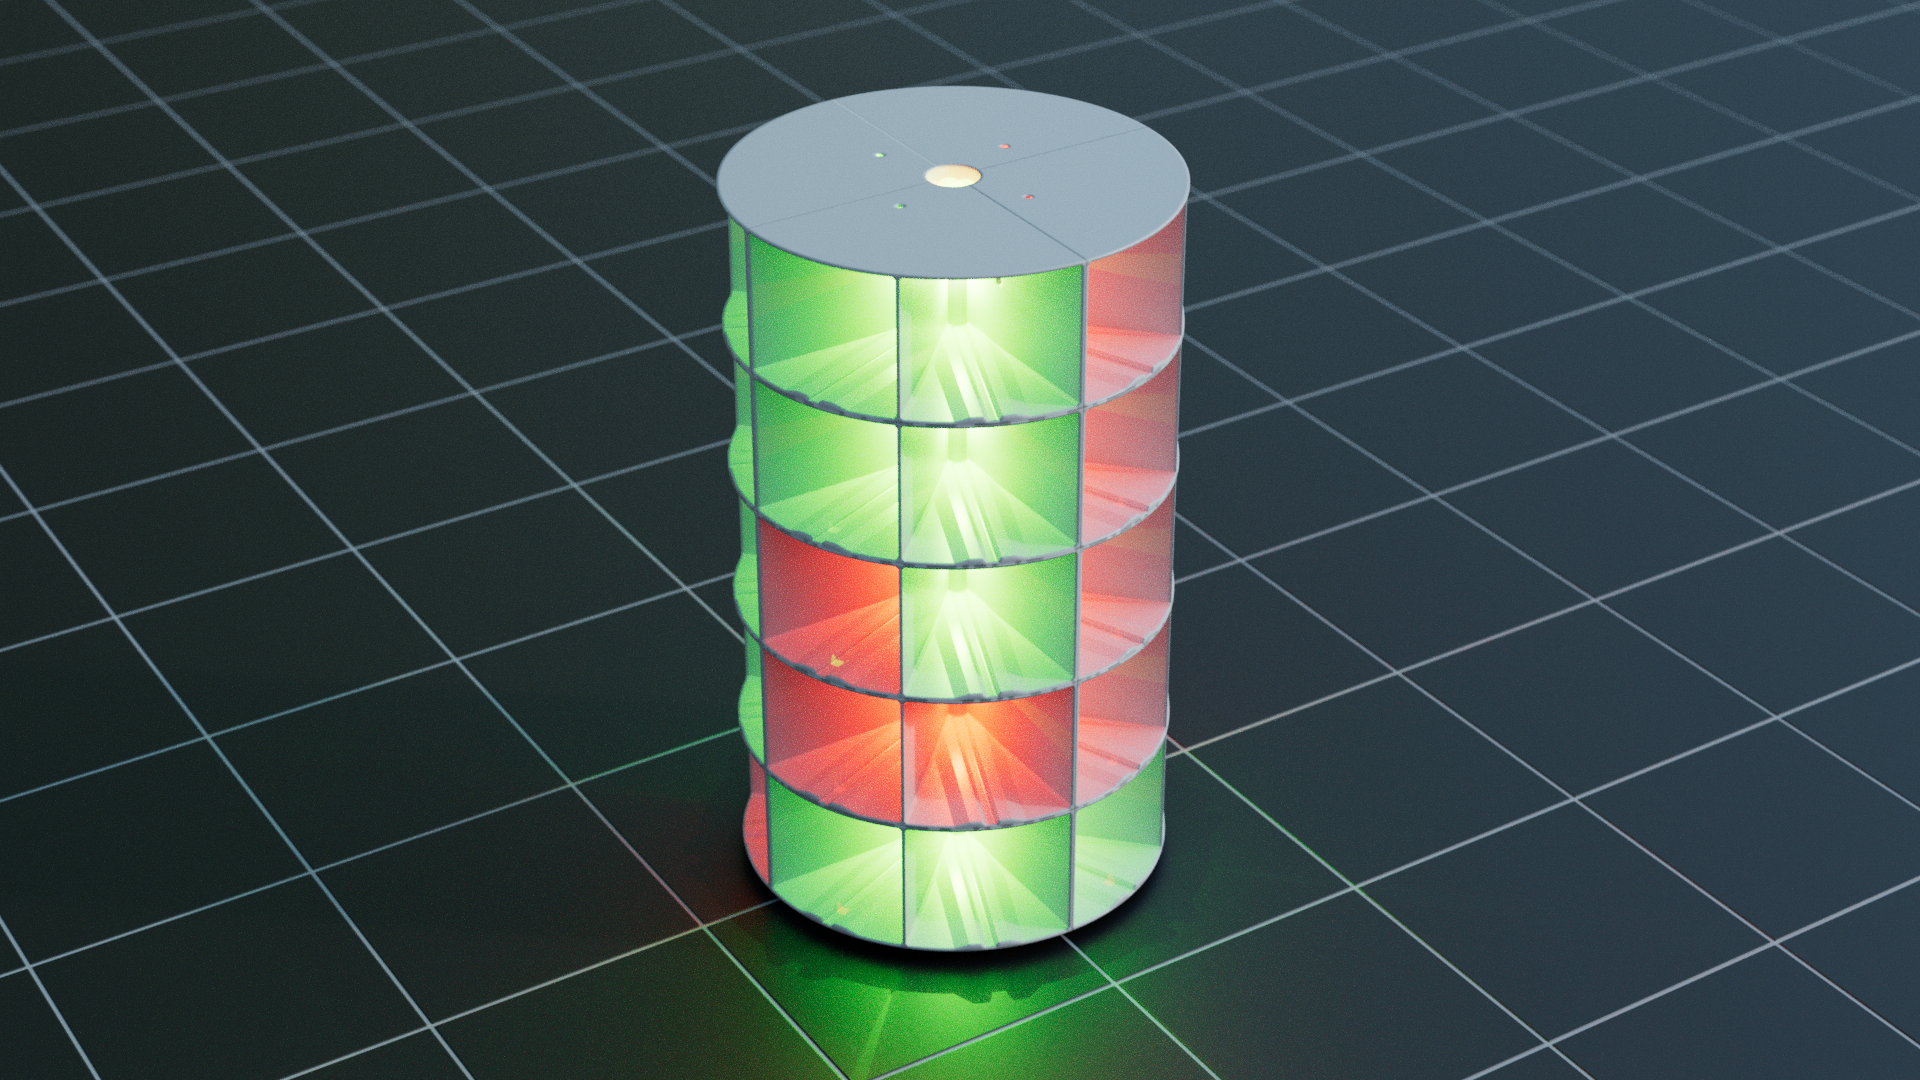
\includegraphics[width=0.8\textwidth]{images/turm_modell.png}
  \caption{Visualisierung des Modell-Turms}
  \label{fig:turm}
\end{figure}